\chapter{O bloco p I: grupos do boro, do carbono e do nitrogênio}\label{ch:b1:p-block-13-15}

O ar que respiramos é composto de quatro quintos de nitrogênio, e no
entanto as plantas passam fome dele: a ligação tripla \ce{N#N} é tão forte
que quase nada a rompe. Durante a maior parte da história, o nitrogênio
das lavouras veio do esterco, de bactérias que vivem nas raízes das
leguminosas e de nitratos extraídos de minas. No início do século XX, uma
reação entre nitrogênio e hidrogênio sobre um \omterm{def:b1:elementary-steps:catalyst}{catalisador} de ferro mudou
isso; hoje o mundo produz cerca de 160 milhões de toneladas de nitrogênio
por ano na forma de amônia, e aproximadamente metade do nitrogênio de um
corpo humano passou por uma fábrica de amônia. Os \omterm{def:b1:periodicity:table}{grupos} 13, 14 e 15
reúnem os elementos dessa história --- nitrogênio e fósforo para os
fertilizantes, carbono e silício para a vida e as rochas, boro e alumínio
para o vidro e as ligas leves. Este capítulo os percorre com as
ferramentas dos capítulos anteriores.

\begin{recall}
Os \omterm{def:b1:crystals-metals:allotropy}{alótropos} do carbono e a estrutura do silício e da sílica
(\cref{ch:b1:crystals-ionic-covalent}); o caráter dos óxidos
(\cref{def:b1:s-block:oxide-character}); os \omterm{def:b1:nernst:oxidation-number}{números de oxidação} e os
\omterm{def:b1:nernst:electrode-potential}{potenciais padrão} (\cref{ch:b1:nernst}); os \omterm{def:b1:precipitation:amphoteric-hydroxide}{hidróxidos anfóteros}
(\cref{ch:b1:precipitation}); as constantes de equilíbrio a partir das
energias de Gibbs (\cref{ch:b1:extent-q-and-k}).
\end{recall}
% ledger: usgs:N-world-2025

\begin{omfigure}
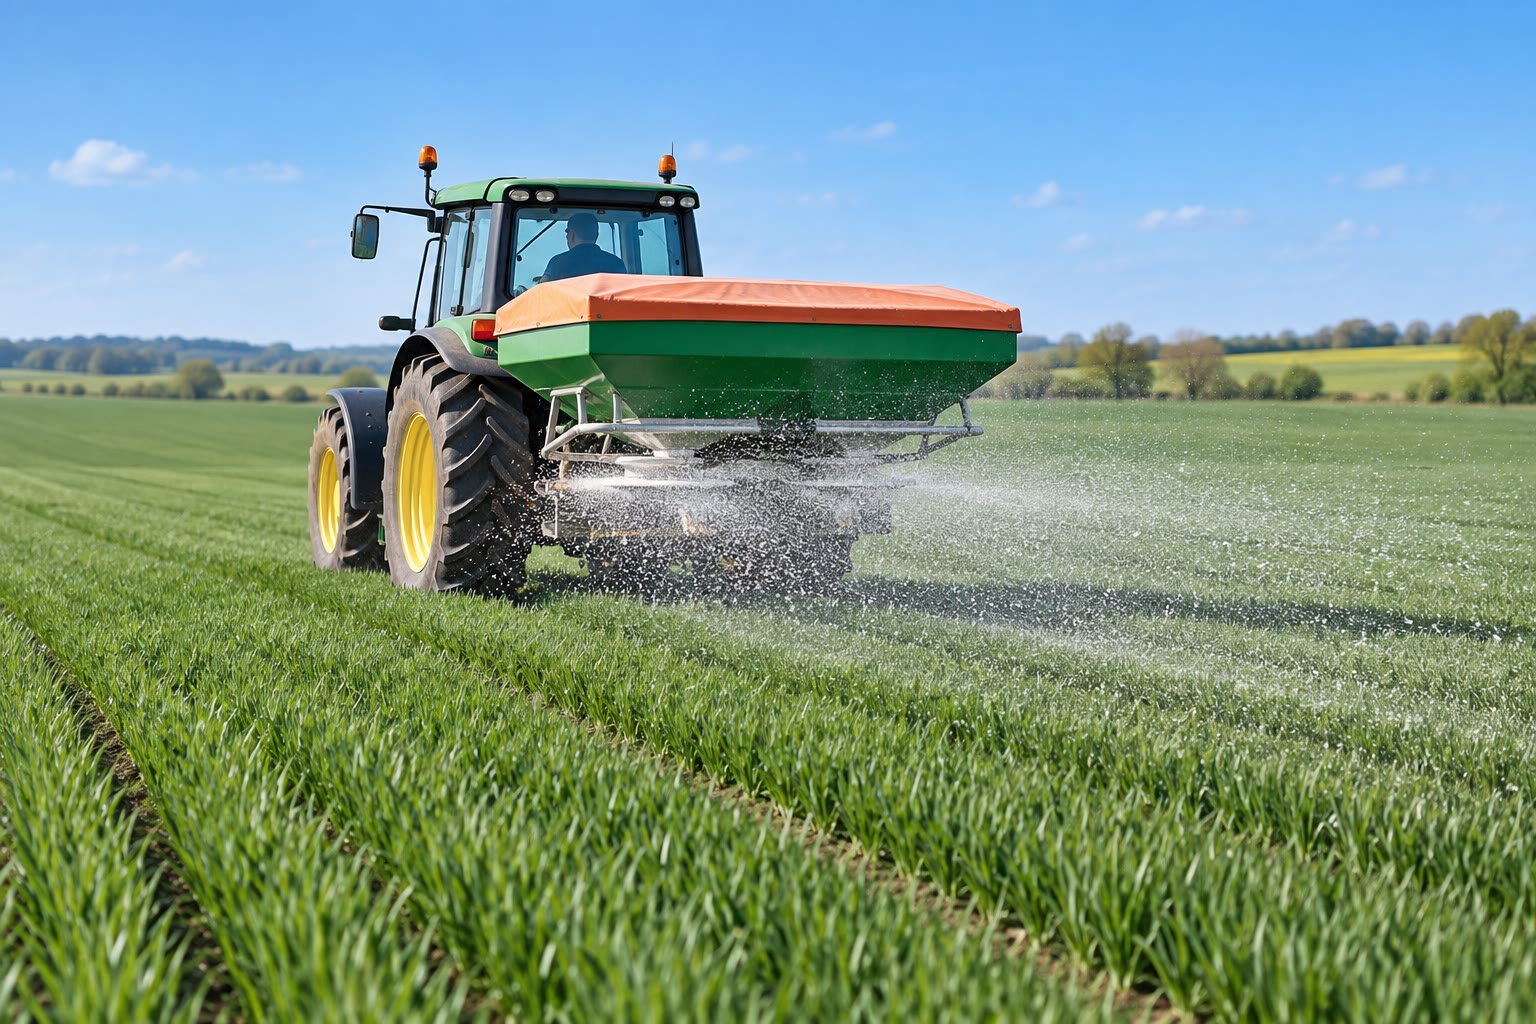
\includegraphics[width=0.55\linewidth]{images/book2/ai/b1-27-fertiliser-field.jpg}

{\small Aplicação de um fertilizante nitrogenado em um campo de trigo. A
maior parte dele foi produzida a partir do nitrogênio do ar pelo processo
Haber--Bosch.}
\end{omfigure}

\section{O grupo 13: o boro e o alumínio}

O boro é um semimetal que forma compostos covalentes com octeto
incompleto: em \ce{BF3} e no ácido bórico \ce{B(OH)3}, o boro tem seis
\omterm{def:b1:quantum-numbers:configuration}{elétrons de valência} e age como \omterm{def:b1:lewis-resonance-vsepr:lewis-acid}{ácido de Lewis} (\cref{ch:b1:lewis-resonance-vsepr}).
O ácido bórico é um \omterm{def:b1:predominant-reaction:strong-acid}{ácido fraco} não por perder um próton, mas por aceitar
um íon hidróxido, \ce{B(OH)3 + 2H2O <=> B(OH)4- + H3O+}. O bórax, um
borato de sódio, é usado em vidros e detergentes.

\begin{definition}[Oxoácido]\label{def:b1:p-block-13-15:oxoacid}
Um \emph{oxoácido}\index{oxoacido@oxoácido} é um ácido em que os átomos de
hidrogênio ácidos estão ligados a átomos de oxigênio ligados a um \omterm{def:b1:complexation:complex}{átomo
central}: \ce{B(OH)3}, \ce{H2CO3}, \ce{HNO3} (\ce{HO-NO2}), \ce{H3PO4}
(\ce{(HO)3PO}), \ce{H2SO4}. Quanto mais átomos de oxigênio sem hidrogênio
em torno do \omterm{def:b1:complexation:complex}{átomo central}, mais forte o ácido.
\end{definition}

O alumínio, abaixo do boro, é um metal, mas seu íon pequeno e muito
carregado lhe dá um óxido e um \omterm{def:b1:precipitation:amphoteric-hydroxide}{hidróxido anfóteros} (\cref{sec:b1:precipitation:amphoteric}).
Seu minério é a bauxita, uma mistura de hidróxidos de alumínio com óxidos
de ferro e sílica; em 2025 o mundo extraiu cerca de 440 milhões de
toneladas de bauxita e refinou a partir dela cerca de 150 milhões de
toneladas de alumina.
% ledger: usgs:bauxite-world-2025, usgs:alumina-world-2025

\begin{proposition}[O processo Bayer]\label{prop:b1:p-block-13-15:bayer}
O hidróxido de sódio concentrado e quente dissolve o alumínio da bauxita
como \ce{Al(OH)4-} e deixa os óxidos de ferro (lama vermelha); resfriar e
semear a solução filtrada precipita \ce{Al(OH)3} puro, calcinado a alumina,
\ce{2Al(OH)3 -> Al2O3 + 3H2O}.
\end{proposition}

\begin{proof}
\ce{Al(OH)3(s) + OH- <=> Al(OH)4-} tem $K = 10^{-1.23}$ a
\qty{25}{\celsius} (\cref{ch:b1:precipitation}): com \ce{[OH-]} alta, o
alumínio fica em solução, enquanto o hidróxido de ferro(III), que não é
anfótero, permanece sólido (\cref{exo:b1:precipitation:12}). A diluição e
o resfriamento baixam \ce{[OH-]} e deslocam o quociente de modo que $Q > K$
para a reação inversa: o hidróxido precipita. A calcinação remove a água.
\end{proof}

A alumina é então reduzida a alumínio por eletrólise em criolita fundida,
uma indústria estudada no volume do 2.º~ano.

\begin{omfigure}
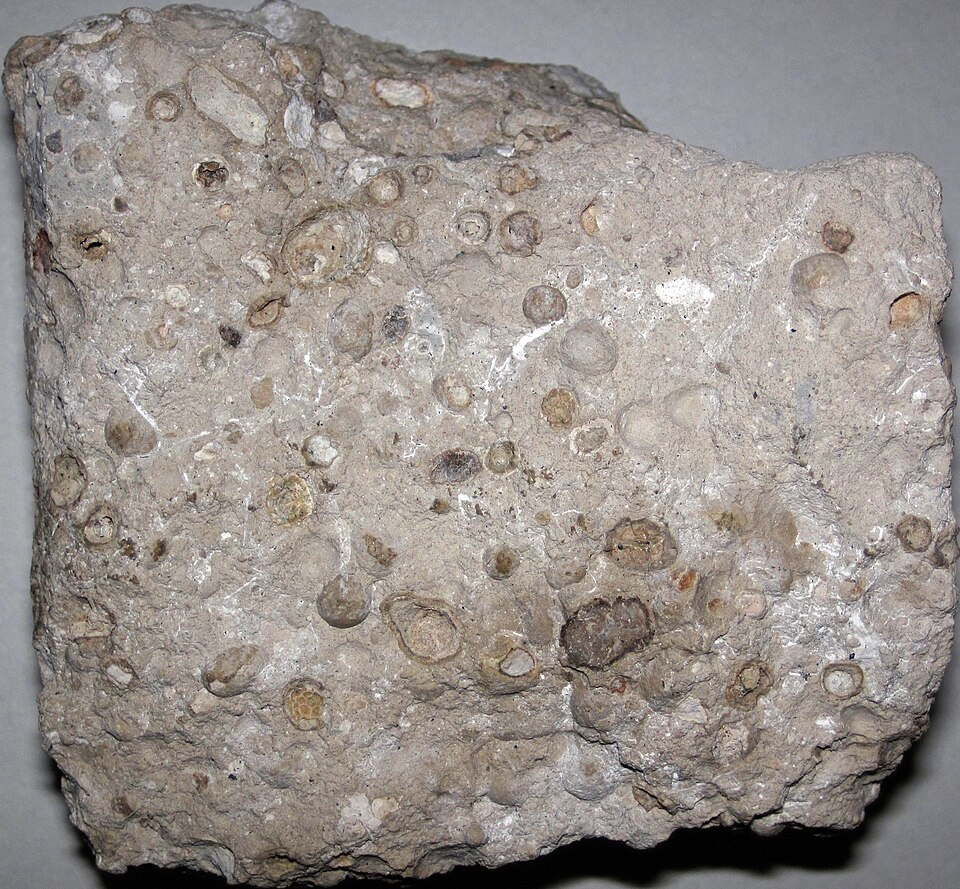
\includegraphics[height=3.6cm]{images/book2/bauxite.jpg}\hspace{0.4em}%
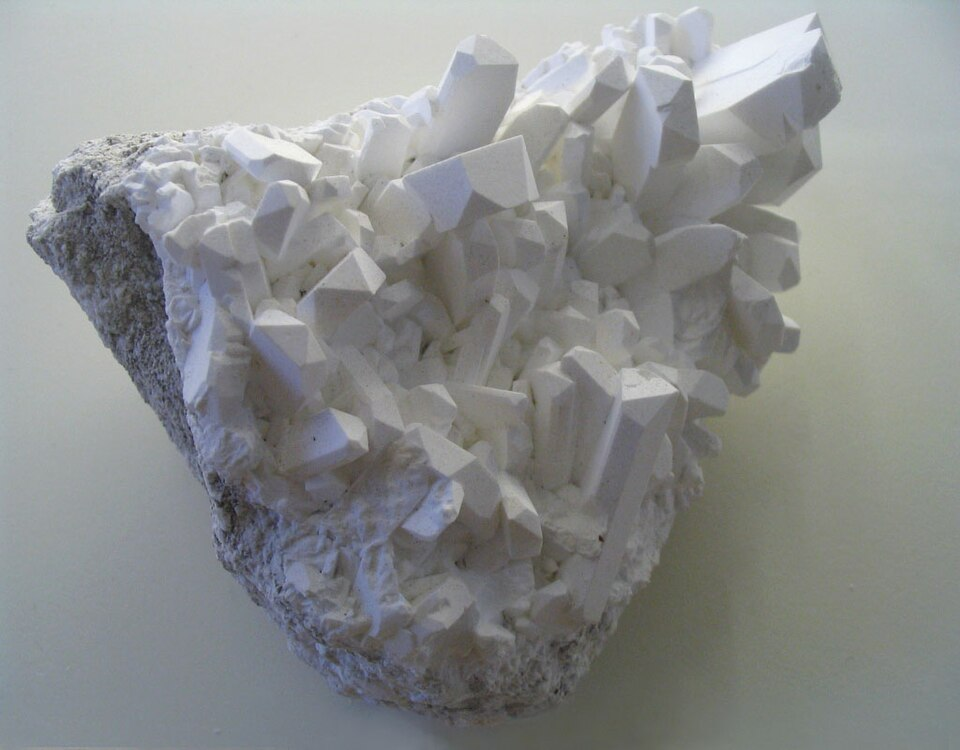
\includegraphics[height=3.6cm]{images/book2/borax.jpg}\hspace{0.4em}%
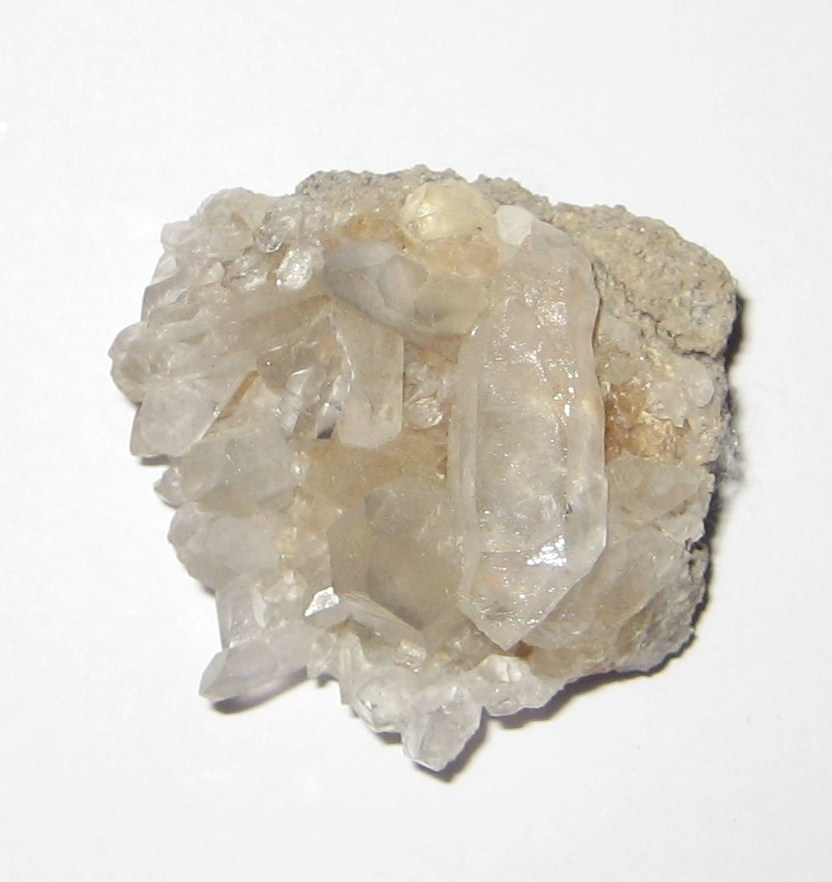
\includegraphics[height=3.6cm]{images/book2/quartz.jpg}\hspace{0.4em}%
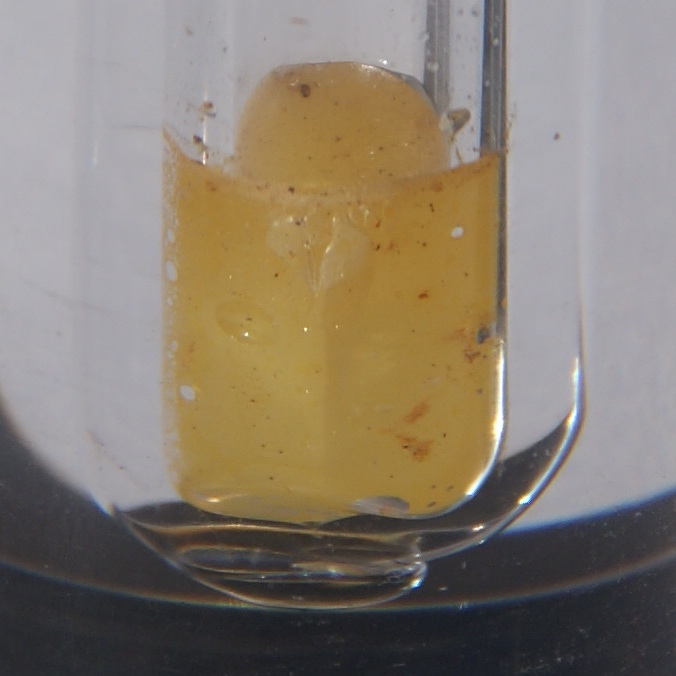
\includegraphics[height=3.6cm]{images/book2/white-phosphorus.jpg}

{\small Da esquerda para a direita: bauxita pisolítica (James St. John,
CC BY 2.0); \omterm{def:b1:crystals-metals:crystal}{cristais} de bórax (Aram Dulyan, domínio público); um
agrupamento de \omterm{def:b1:crystals-metals:crystal}{cristais} de quartzo, \ce{SiO2} (Stephanie Clifford, CC BY
2.0); fósforo branco, com um pouco de fósforo vermelho, guardado sob água
porque se inflama no ar (Hi-Res Images of Chemical Elements, CC BY 3.0).
Todas da Wikimedia Commons.}
\end{omfigure}

\section{O grupo 14: o carbono e o silício}

O carbono e o silício formam ambos quatro ligações, mas de modo
diferente. O carbono forma ligações duplas fortes: \ce{CO2} é uma
molécula, \ce{O=C=O}, um gás. O silício quase não as forma: \ce{SiO2} é
uma rede covalente de tetraedros \ce{SiO4} que compartilham todos os seus
vértices, um sólido duro, o quartzo (\cref{ch:b1:crystals-ionic-covalent}).
O dióxido de carbono é um \omterm{def:b1:s-block:oxide-character}{óxido ácido}, que dá ácido carbônico,
hidrogenocarbonatos e carbonatos (\cref{ch:b1:predominant-reaction}); a
sílica também é um \omterm{def:b1:s-block:oxide-character}{óxido ácido}, atacado por álcalis fundidos dando silicatos.

\begin{proposition}[Unidades silicato]\label{prop:b1:p-block-13-15:silicate-units}
Os silicatos são construídos com tetraedros \ce{SiO4}; o número de
vértices compartilhados com outros tetraedros fixa a fórmula do ânion:
nenhum, \ce{SiO4^4-} (tetraedros isolados); dois, cadeias $(\ce{SiO3})_n^{2n-}$;
três, folhas $(\ce{Si2O5})_n^{2n-}$; quatro, a estrutura tridimensional
neutra \ce{SiO2}.
\end{proposition}

\begin{proof}
Um oxigênio compartilhado pertence metade a cada tetraedro. Um tetraedro
que compartilha $k$ vértices possui $4 - k$ átomos de oxigênio por
inteiro e $k$ pela metade: $4 -
k/2$ oxigênios por silício. Cada oxigênio não compartilhado leva uma
carga $-1$ (tem uma única ligação), cada compartilhado nenhuma: a carga
por silício é $-(4 - k)$. $k = 0$: \ce{SiO4^4-}; $k = 2$: \ce{SiO3^2-} por
silício; $k = 3$: \ce{SiO_{2.5}^-}, isto é, \ce{Si2O5^2-}; $k = 4$: \ce{SiO2}.
\end{proof}

\begin{omfigure}
\begin{tikzpicture}[font=\small, line join=round]
  % um tetraedro SiO4 em perspectiva
  \begin{scope}
    \coordinate (t) at (0,1.2); \coordinate (a) at (-1.0,-0.5);
    \coordinate (b) at (1.0,-0.5); \coordinate (c) at (0.25,0.05);
    \draw[thick, omDef] (t) -- (a) -- (b) -- cycle; \draw[thick, omDef] (t) -- (b);
    \draw[dashed, omDef] (a) -- (c) -- (b) (t) -- (c);
    \foreach \p in {t,a,b,c} \shade[ball color=red!60] (\p) circle (0.16);
    \shade[ball color=gray!40] (0.06,0.18) circle (0.11);
    \node at (0,-1.2) {\ce{SiO4^4-}: um tetraedro};
  \end{scope}
  % uma cadeia de tetraedros vista de cima
  \begin{scope}[xshift=3.6cm]
    \foreach \i in {0,1,2,3} {
      \draw[thick, omDef, fill=omDef!10] (\i*1.1,0) -- (\i*1.1+0.55,0.95) -- (\i*1.1+1.1,0) -- cycle;
      \shade[ball color=red!60] (\i*1.1+0.55,0.95) circle (0.12);
      \shade[ball color=red!60] (\i*1.1+0.55,0.32) circle (0.10);
    }
    \foreach \i in {0,1,2,3,4} \shade[ball color=red!60] (\i*1.1,0) circle (0.12);
    \node[align=center] at (2.2,-1.0) {cadeia $(\ce{SiO3})_n^{2n-}$: cada tetraedro\\ compartilha dois vértices (vista de cima)};
  \end{scope}
\end{tikzpicture}

{\small Unidades silicato: um tetraedro \ce{SiO4} isolado (silício em
cinza, oxigênio em vermelho) e uma cadeia em que cada tetraedro
compartilha dois átomos de oxigênio com seus vizinhos. As folhas (três
vértices compartilhados) formam as micas e as argilas; a estrutura
tridimensional (quatro), o quartzo.}
\end{omfigure}

\begin{definition}[Efeito do par inerte]\label{def:b1:p-block-13-15:inert-pair}
O \emph{efeito do par inerte}\index{efeito do par inerte} é a estabilidade
crescente, descendo os \omterm{def:b1:periodicity:table}{grupos} 13 a 15, do estado de oxidação duas unidades
abaixo do mais alto do grupo: tálio(I) em vez de (III), chumbo(II) em vez
de (IV), bismuto(III) em vez de (V). O par \textit{ns}$^2$ dos elementos
pesados é mantido firmemente e pouco participa das ligações.
\end{definition}

O efeito explica por que o óxido de chumbo(IV) é um \omterm{def:b1:nernst:couple}{oxidante} forte
($E^\circ(\ce{PbO2}/\ce{Pb^2+}) = 1.46$~V, \cref{ch:b1:nernst}), enquanto
o carbono(IV) e o silício(IV) são os estados estáveis de seus elementos.

\section{O grupo 15: o nitrogênio}

\begin{proposition}[A escada do nitrogênio]\label{prop:b1:p-block-13-15:nitrogen-ladder}
O nitrogênio assume todos os \omterm{def:b1:nernst:oxidation-number}{números de oxidação} de $-3$ a $+5$: \ce{NH3} e
\ce{NH4+} ($-$III), \ce{N2H4} ($-$II), \ce{NH2OH} ($-$I), \ce{N2} (0),
\ce{N2O} ($+$I), \ce{NO} ($+$II), \ce{HNO2} e \ce{NO2-} ($+$III),
\ce{NO2} ($+$IV), \ce{HNO3} e \ce{NO3-} ($+$V).
\end{proposition}

\begin{proof}
Aplique as regras da \cref{prop:b1:nernst:on-rules} a cada fórmula, com H
em $+$I e O em $-$II: em \ce{N2H4}, $2x + 4 = 0$; em \ce{NO2-}, $x - 4 =
-1$; e assim por diante.
\end{proof}

\begin{definition}[Fixação do nitrogênio]\label{def:b1:p-block-13-15:nitrogen-fixation}
A \emph{fixação do nitrogênio}\index{fixacao do nitrogenio@fixação do nitrogênio} é todo processo que
converte o dinitrogênio do ar em um composto (amônia, nitrato) que os
organismos vivos ou a indústria podem usar: fixação biológica por
bactérias, fixação pelos raios e a síntese industrial da amônia.
\end{definition}

O processo Haber--Bosch combina nitrogênio e hidrogênio sobre um
\omterm{def:b1:elementary-steps:catalyst}{catalisador} de ferro, \ce{N2 + 3H2 <=> 2NH3}. A reação é favorecida à
temperatura ambiente ($K = 10^{5.8}$ a \qty{25}{\celsius}, a partir da
energia de Gibbs de formação da amônia), mas é lenta demais; o \omterm{def:b1:elementary-steps:catalyst}{catalisador}
só funciona a quente, e a escolha de temperatura e pressão que concilia
velocidade e \omterm{def:b1:extent-q-and-k:fractional-extent}{rendimento} é feita no volume do 2.º~ano. A amônia é então
oxidada a ácido nítrico pelo processo Ostwald.
% ledger: dfg:NH3_g

\begin{omfigure}
\begin{tikzpicture}[font=\small, >={Stealth}, box/.style={draw, rounded corners, fill=omDef!8, align=center, minimum height=0.9cm}]
  \node[box] (air) at (0,0) {ar\\\ce{N2}};
  \node[box] (gas) at (0,-1.6) {gás natural\\\ce{H2}};
  \node[box] (hb) at (3.4,-0.8) {Haber--Bosch\\catalisador\\de ferro};
  \node[box] (ox1) at (7.3,-0.8) {tela\\de Pt--Rh\\\ce{NH3} $\to$ \ce{NO}};
  \node[box] (ox2) at (11.0,-0.8) {oxidação\\absorção\\\ce{NO} $\to$ \ce{NO2} $\to$ \ce{HNO3}};
  \draw[->, thick] (air) -- (hb);
  \draw[->, thick] (gas) -- (hb);
  \draw[->, thick] (hb) -- node[above] {\ce{NH3}} (ox1);
  \draw[->, thick] (ox1) -- node[above] {\ce{NO}} (ox2);
  \draw[->, thick] (ox2.south) -- ++(0,-0.6) node[below] {\ce{HNO3}};
  \draw[->, thick] (hb.south) -- ++(0,-0.9) node[below] {\ce{NH3} (fertilizantes)};
  \draw[->, thick] (ox2.north) -- ++(0,0.5) -| node[pos=0.25, above] {\ce{NO} reciclado} (ox1.north);
\end{tikzpicture}

{\small Do ar ao ácido nítrico: a síntese da amônia seguida das três
etapas do processo Ostwald.}
\end{omfigure}

\begin{method}[Balancear equações industriais encadeadas]\label{met:b1:p-block-13-15:ostwald-balance}
\begin{enumerate}
  \item Balanceie cada etapa: (1) \ce{4NH3 + 5O2 -> 4NO + 6H2O};
        (2) \ce{2NO + O2 -> 2NO2}; (3) \ce{3NO2 + H2O -> 2HNO3 + NO}.
  \item Multiplique as etapas de modo que cada intermediário formado seja
        consumido (o \ce{NO} da etapa 3 volta à etapa 2).
  \item Some: com reciclagem completa do NO, a equação global é
        \ce{NH3 + 2O2 -> HNO3 + H2O}, um ácido nítrico por amônia.
  \item Use a equação global para os balanços de massa, e as etapas para
        o projeto de cada reator.
\end{enumerate}
\end{method}

\begin{history}[Fritz Haber]
\begin{minipage}[t]{0.18\linewidth}\vspace{0pt}
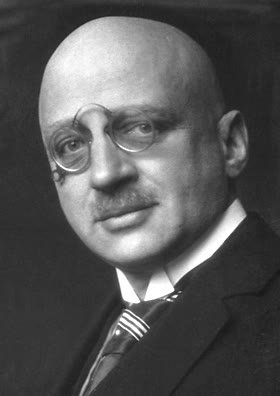
\includegraphics[width=\linewidth]{images/book2/haber.jpg}
\end{minipage}\hfill
\begin{minipage}[t]{0.78\linewidth}\vspace{0pt}
Fritz Haber mostrou que a amônia podia ser obtida a partir de nitrogênio
e hidrogênio sob pressão sobre um \omterm{def:b1:elementary-steps:catalyst}{catalisador}; Carl Bosch transformou a
reação de laboratório em um processo industrial. Haber recebeu o Prêmio
Nobel de Química de 1918. O mesmo homem dirigiu o primeiro uso em grande
escala do cloro como arma, na Primeira Guerra Mundial: a química que
alimenta metade da humanidade e a química que mata estão separadas pelas
escolhas dos químicos.
(Fotografia: The Nobel Foundation, publicada em 1919, domínio público,
Wikimedia Commons.)
\end{minipage}
\end{history}

\section{O fósforo e as tendências ao longo dos grupos}

O fósforo, abaixo do nitrogênio, não forma ligações triplas \ce{P#P}: o
fósforo branco é formado por tetraedros \ce{P4}, tensionados e reativos
(ele se inflama no ar e é guardado sob água); o fósforo vermelho é um
polímero, muito menos reativo. A combustão do fósforo dá \ce{P4O10}, o
mais ácido dos óxidos comuns, que com a água dá o ácido fosfórico,
$\mathrm{p}K_a$ 2.15, 7.21, 12.34 (\cref{ch:b1:predominant-reaction}).
A rocha fosfática, extraída na ordem de 250 milhões de toneladas em 2025,
é transformada pelo ácido sulfúrico em fertilizantes fosfatados.
% ledger: usgs:phosphate-world-2025

Descendo cada grupo, os elementos se tornam mais metálicos (do boro ao
tálio, do carbono ao chumbo, do nitrogênio ao bismuto), seus óxidos mais
básicos, e os estados de oxidação mais baixos mais estáveis: o \omterm{def:b1:p-block-13-15:inert-pair}{efeito do
par inerte}. Ao longo de um \omterm{def:b1:periodicity:table}{período}, os óxidos se tornam mais ácidos, do
\ce{Na2O} básico aos \omterm{def:b1:s-block:oxide-character}{óxidos ácidos} do fósforo e do enxofre.

\section{Exercícios}

\begin{exercise}[$\star$]\label{exo:b1:p-block-13-15:1}
Dê o \omterm{def:b1:nernst:oxidation-number}{número de oxidação} do nitrogênio em \ce{NH4NO3} (os dois átomos),
\ce{N2O5}, \ce{HNO2}, \ce{N2H4} e \ce{Mg3N2}.
\end{exercise}

\begin{exercise}[$\star$]\label{exo:b1:p-block-13-15:2}
Desenhe as \omterm{def:b1:lewis-resonance-vsepr:lewis}{estruturas de Lewis} de \ce{BF3}, de \ce{NH3} e do aduto
\ce{F3B-NH3}; identifique o ácido e a \omterm{def:b1:lewis-resonance-vsepr:lewis-acid}{base de Lewis}.
\end{exercise}

\begin{exercise}[$\star$]\label{exo:b1:p-block-13-15:3}
Escreva as reações de \ce{CO2}, \ce{SiO2} (fundido) e \ce{P4O10} com o
hidróxido de sódio, e de \ce{Al2O3} com um ácido e com uma base.
\end{exercise}

\begin{exercise}[$\star$]\label{exo:b1:p-block-13-15:4}
Calcule a constante de equilíbrio de \ce{N2 + 3H2 <=> 2NH3} a
\qty{25}{\celsius} a partir de $\Delta_f G^\circ(\ce{NH3}) =
\qty{-16.45}{kJ/mol}$.
\end{exercise}

\begin{exercise}[$\star\star$]\label{exo:b1:p-block-13-15:5}
Usando a contagem da \cref{prop:b1:p-block-13-15:silicate-units}, dê a
fórmula de um anel de seis tetraedros que compartilham cada um dois
vértices (como no berilo) e de uma cadeia dupla em que metade dos
tetraedros compartilha dois vértices e a outra metade, três.
\end{exercise}

\begin{exercise}[$\star\star$]\label{exo:b1:p-block-13-15:6}
Calcule a massa de alumina obtida a partir de uma tonelada de bauxita
contendo \qty{55}{\percent} em massa de \ce{Al(OH)3}, com recuperação de
\qty{92}{\percent}.
\end{exercise}

\begin{exercise}[$\star\star$]\label{exo:b1:p-block-13-15:7}
Mostre que o ácido bórico é um \omterm{def:b1:lewis-resonance-vsepr:lewis-acid}{ácido de Lewis} e não um \omterm{def:b1:predominant-reaction:bronsted}{ácido de Brønsted},
e explique por que sua solução é, ainda assim, ácida.
\end{exercise}

\begin{exercise}[$\star\star$]\label{exo:b1:p-block-13-15:8}
Balanceie a oxidação da amônia a \ce{NO} com os \omterm{def:b1:nernst:oxidation-number}{números de oxidação} e dê
o número de elétrons trocados por \ce{NH3}.
\end{exercise}

\begin{exercise}[$\star\star$]\label{exo:b1:p-block-13-15:9}
O nitrato de amônio é produzido a partir de amônia e ácido nítrico.
Escreva a reação e calcule a massa de amônia necessária (tanto para o
ácido nítrico quanto para a neutralização) por tonelada de nitrato de amônio.
\end{exercise}

\begin{exercise}[$\star\star\star$]\label{exo:b1:p-block-13-15:10}
Explique por que o nitrogênio é um gás diatômico e o fósforo um sólido de
moléculas \ce{P4}, e por que o dióxido de carbono é um gás e a sílica um
sólido, usando a força das ligações $\pi$ entre átomos do segundo e do
terceiro \omterm{def:b1:periodicity:table}{períodos}.
\end{exercise}

\begin{exercise}[$\star\star\star$]\label{exo:b1:p-block-13-15:11}
Mostre com os \omterm{def:b1:nernst:electrode-potential}{potenciais padrão} que o óxido de chumbo(IV) oxida os íons
cloreto a cloro em meio ácido, enquanto o óxido de silício(IV) não faz
nada disso. Relacione isso com o \omterm{def:b1:p-block-13-15:inert-pair}{efeito do par inerte}.
\end{exercise}

\begin{exercise}[$\star\star\star$]\label{exo:b1:p-block-13-15:12}
O mundo produziu cerca de 160 milhões de toneladas de nitrogênio na forma
de amônia em 2025. Que massa de amônia é essa, e que massa de hidrogênio
ela continha? De onde vem principalmente esse hidrogênio?
\end{exercise}

\section{Problema: do ar ao fertilizante}

\begin{problem}[{Problema de fim de semana --- a ligação tripla do
nitrogênio, a síntese da amônia, as três etapas da fabricação do ácido
nítrico, o nitrato de amônio, e a massa de ácido nítrico obtida a partir
de uma tonelada de amônia}]
\label{pb:b1:p-block-13-15:1}
Uma fábrica de fertilizantes converte amônia em ácido nítrico e em
nitrato de amônio. Massas molares (\unit{g/mol}): \ce{N2} 28.0, \ce{H2} 2.0, \ce{NH3}
17.0, \ce{HNO3} 63.0, \ce{NH4NO3} 80.0, \ce{O2} 32.0;
$\Delta_f G^\circ(\ce{NH3(g)}) = \qty{-16.45}{kJ/mol}$ a
\qty{25}{\celsius}.

\medskip
\noindent\textbf{Parte I --- O nitrogênio.}
\begin{enumerate}
  \item Desenhe a \omterm{def:b1:lewis-resonance-vsepr:lewis}{estrutura de Lewis} de \ce{N2} e diga por que ele é pouco reativo.
  \item Dê o \omterm{def:b1:nernst:oxidation-number}{número de oxidação} de N em \ce{N2}, \ce{NH3}, \ce{NO},
        \ce{NO2}, \ce{HNO3} e \ce{NH4NO3}.
  \item Cite três modos, naturais ou industriais, de fixar o nitrogênio.
  \item Por que as plantas não conseguem usar \ce{N2} diretamente?
  \item Que elemento é oxidado e qual é reduzido na síntese da
        amônia?
  \item Escreva a síntese da amônia.
\end{enumerate}

\medskip
\noindent\textbf{Parte II --- A amônia.}
\begin{enumerate}[resume]
  \item Calcule a constante de equilíbrio da síntese a
        \qty{25}{\celsius}.
  \item Por que a síntese é, ainda assim, feita a quente, sobre um \omterm{def:b1:elementary-steps:catalyst}{catalisador}?
  \item Calcule as massas de \ce{N2} e de \ce{H2} para uma tonelada de
        amônia.
  \item Que volume de ar (\qty{78}{\percent} de \ce{N2} em volume, gás
        ideal, \qty{25}{\celsius}, \qty{1}{bar}) contém esse nitrogênio?
  \item De onde vem o hidrogênio?
  \item Por que a própria amônia é usada como fertilizante em alguns
        países, e por que ela é muitas vezes convertida antes?
\end{enumerate}

\medskip
\noindent\textbf{Parte III --- O ácido nítrico.}
\begin{enumerate}[resume]
  \item Balanceie a etapa 1, \ce{NH3 + O2 -> NO + H2O}, com os \omterm{def:b1:nernst:oxidation-number}{números de oxidação}. % ce-unbalanced-ok
  \item Balanceie a etapa 2, \ce{NO + O2 -> NO2}. % ce-unbalanced-ok
  \item Balanceie a etapa 3, \ce{NO2 + H2O -> HNO3 + NO}. Que tipo de % ce-unbalanced-ok
        reação de oxirredução é essa?
  \item Combine as etapas, com reciclagem completa do NO, na equação
        global.
  \item Calcule a massa de oxigênio consumida por tonelada de amônia.
  \item Por que se usa uma tela de platina--ródio na etapa 1?
\end{enumerate}

\medskip
\noindent\textbf{Parte IV --- O nitrato de amônio e os balanços de massa.}
\begin{enumerate}[resume]
  \item Escreva a formação do nitrato de amônio.
  \item Que fração da amônia deve ser transformada em ácido nítrico para
        produzir apenas nitrato de amônio?
  \item Calcule a massa de nitrato de amônio obtida a partir de uma
        tonelada de amônia repartida dessa maneira.
  \item Que porcentagem de nitrogênio o nitrato de amônio contém?
  \item Por que o nitrato de amônio deve ser guardado longe de
        combustíveis e do calor?
  \item Calcule a massa de ácido nítrico que se pode obter a partir de
        uma tonelada de amônia (conversão completa).
\end{enumerate}
\end{problem}
